%----------------------------------------------------------------------------------------
%	PACKAGES AND THEMES
%----------------------------------------------------------------------------------------
\documentclass[aspectratio=169,xcolor=dvipsnames, t]{beamer}
\usepackage{fontspec} % Allows using custom font. MUST be before loading the theme!
\usetheme{SimplePlusAIC}
\usepackage{hyperref}
\usepackage{graphicx} % Allows including images
\usepackage{booktabs} % Allows the use of \toprule, \midrule and  \bottomrule in tables
\usepackage{svg} %allows using svg figures
\usepackage{tikz}
\usepackage{makecell}
\usepackage{wrapfig}
% ADD YOUR PACKAGES BELOW
\usepackage{subcaption}

%----------------------------------------------------------------------------------------
%	TITLE PAGE CONFIGURATION
%----------------------------------------------------------------------------------------

\title[Machine Learning]{Modèles linguistiques : Machine Learning } % The short title appears at the bottom of every slide, the full title is only on the title page
\subtitle{Classification}

\author{Luis Moreno}
\institute[Sorbonne Université]{UFR de Sociologie et d'Informatique pour les Sciences Humaines 
\newline
Sorbonne Université
}
% Your institution as it will appear on the bottom of every slide, maybe shorthand to save space


\date{\today} % Date, can be changed to a custom date
%----------------------------------------------------------------------------------------
%	PRESENTATION SLIDES
%----------------------------------------------------------------------------------------

\begin{document}

\maketitlepage

\begin{frame}[t]{Agenda}
    % Throughout your presentation, if you choose to use \section{} and \subsection{} commands, these will automatically be printed on this slide as an overview of your presentation
    \tableofcontents
\end{frame}

%------------------------------------------------
% Section divider frame
\makesection{Introduction}
%------------------------------------------------
\begin{frame}{Classification ?}
	\begin{itemize}
		\item Une tâche classique en apprentissage automatique (\textit{Machine Learning}).
		\item Par exemple :
		\begin{itemize}
			\item Donné une image comme entrée
			\item Prédire le nombre dans l'image
		\end{itemize}
	\end{itemize}
	
	\begin{figure}
		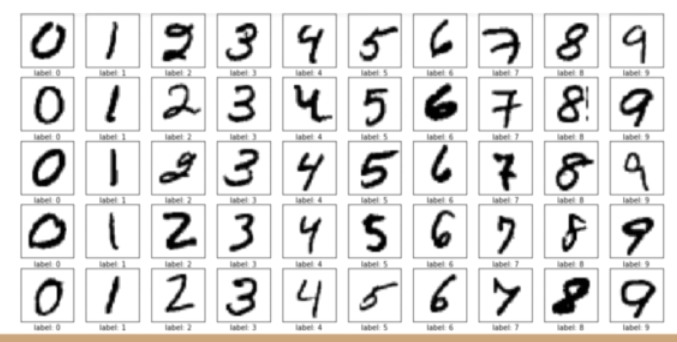
\includegraphics[height=0.4\paperheight ]{figures/cm2_ClassificationImages.png}
	\end{figure}
\end{frame}

%------------------------------------------------

\begin{frame}{Données fréquentes en classification}
	\begin{itemize}
		\item Images -- Vision artificielle
		\item Texte -- Traitement Automatiques de Langues
		\item Les données le plus traitées actuellement.
	\end{itemize}
	\textbf{Exemple de classification de texte :}
	\begin{itemize}
		\item Spam
		\item Sentiments
		\item Polarité - avis, commentaire, ...
	\end{itemize}

\end{frame}
%------------------------------------------------

\begin{frame}{À retenir !}
	Le fonctionement des modèles en ML :
	\begin{enumerate}
		\item Input
		\begin{itemize}
			\item texte
			\item images
			\item vidéos
			\item audio
		\end{itemize}
		\item ML modèle
		\begin{itemize}
			\item classification
			\item clustering 
			\item RN
		\end{itemize}
		\item Prédiction 
		\begin{itemize}
			\item binaire - classification
			\item approximation - régression linaire
		\end{itemize}
	\end{enumerate}
\end{frame}
%------------------------------------------------
\begin{frame}{Comment le modèle apprend ?}
\begin{itemize}
	\item Comment le modèle apprend a faire de prédictions
	\item Comment sont elles traitées les données
	\begin{itemize}
		\item Données d'entrées (caractéristiques - \textbf{X}) et d'étiquettes (target - \textbf{Y})
		\item Extraction de caractéristiques 
	\end{itemize}
\end{itemize}

\begin{figure}
	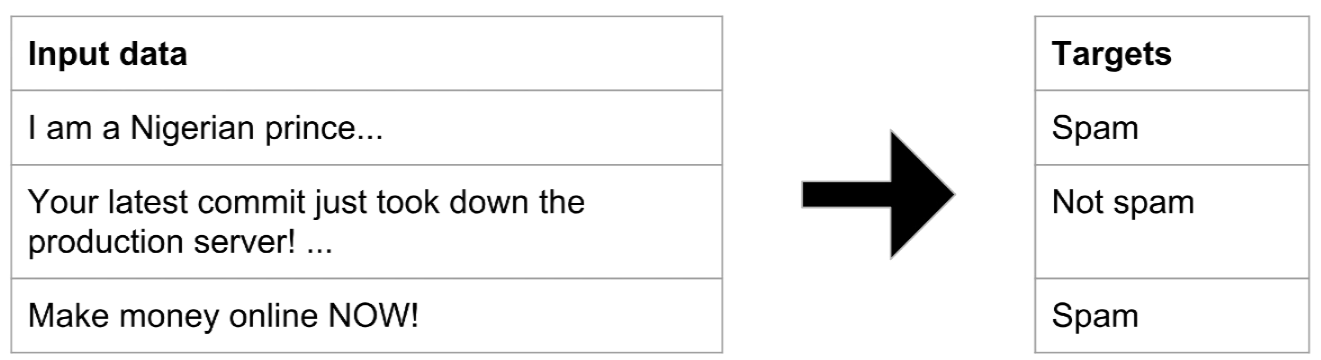
\includegraphics[height=0.4\paperheight ]{figures/cm2_InputClassification.png}
\end{figure}
\end{frame}
%------------------------------------------------
\begin{frame}{Comment le modèle apprend ?}
\begin{itemize}
	\item Traitons les données !
	\item Si nous avons
	\begin{itemize}
		\item \textbf{X} (une matrice de $N \times D $) Important ! la matrice contient que des valeurs numériques.
		\begin{itemize}
			\item $N$ = nombre de données d'entraînement
			\item $D$ = nombre de caractéristiques
		\end{itemize}
		\item \textbf{Y} (un vecteur de taille $N$ contenant les étiquettes (targets)
	\end{itemize}
\end{itemize}

	\begin{figure}
		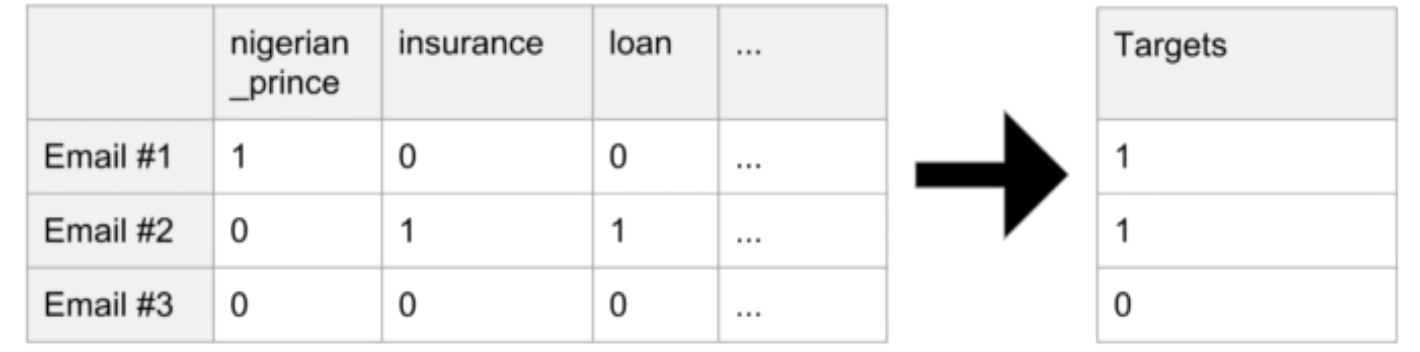
\includegraphics[height=0.35\paperheight ]{figures/cm2_InputClassification2.png}
	\end{figure}
\end{frame}
%------------------------------------------------
\begin{frame}{Le code}
	
	
	\begin{example}[\textbf{Implémentation}]
		import RandomForestClassifier from sklearn\\
		
		model = RandomForestClassifier() \#Charger le modèle\\
		
		model.fit(X,Y) \#Apprentissage\\
		
		prediction = model.predict(X)
	\end{example}
	
	\begin{example}[\textbf{Évaluation}]
		
		precision = total\_correct / totals\\
		
		model.score(X,Y)
	\end{example}

\end{frame}

%------------------------------------------------
% Section divider frame
\makesection{Not magic, juste un problème géométrique}
%------------------------------------------------
\begin{frame}{Régression linaire}
	Le but c'est du trouver la ligne que mieux décrit les données analysées
	\begin{figure}
		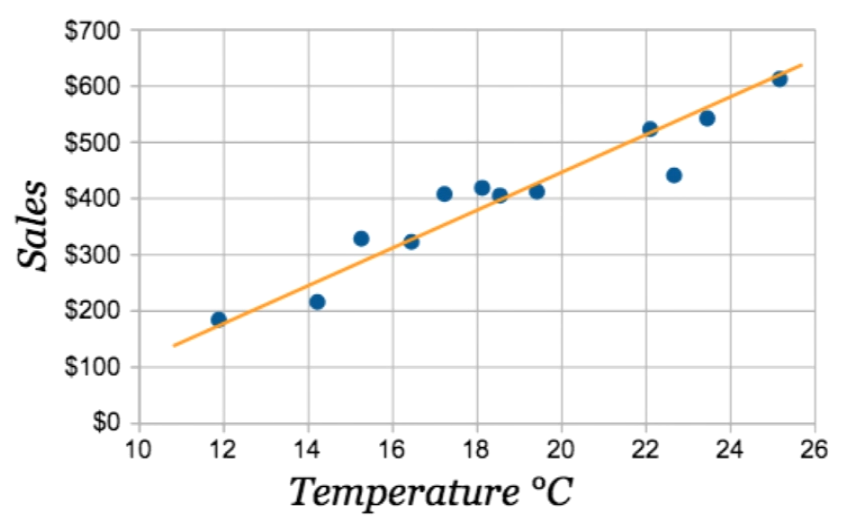
\includegraphics[height=0.6\paperheight ]{figures/cm2_notMagic.png}
	\end{figure}
	
\end{frame}%------------------------------------------------
\begin{frame}{Régression linaire}
Mais pas tout le temps est si simple
\begin{figure}
	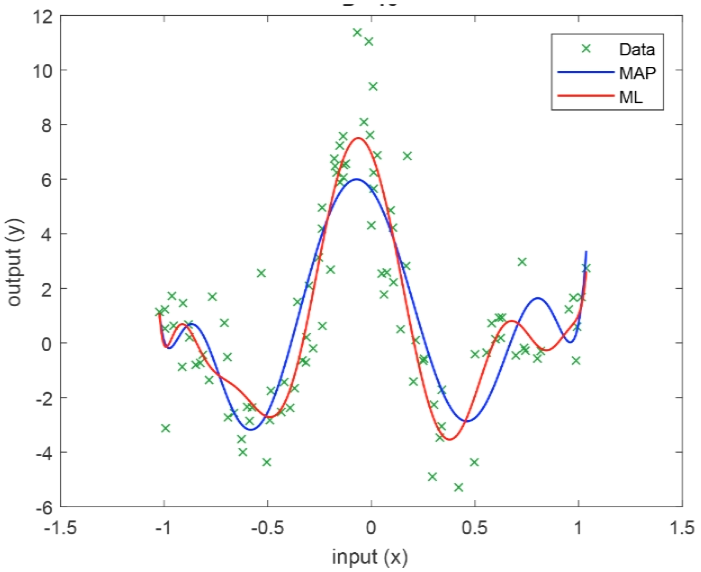
\includegraphics[height=0.6\paperheight ]{figures/cm2_notMagic2.png}
\end{figure}

Et ça peut se compliquer encore plus !
\end{frame}

\begin{frame}{Classification}
	\begin{figure}
		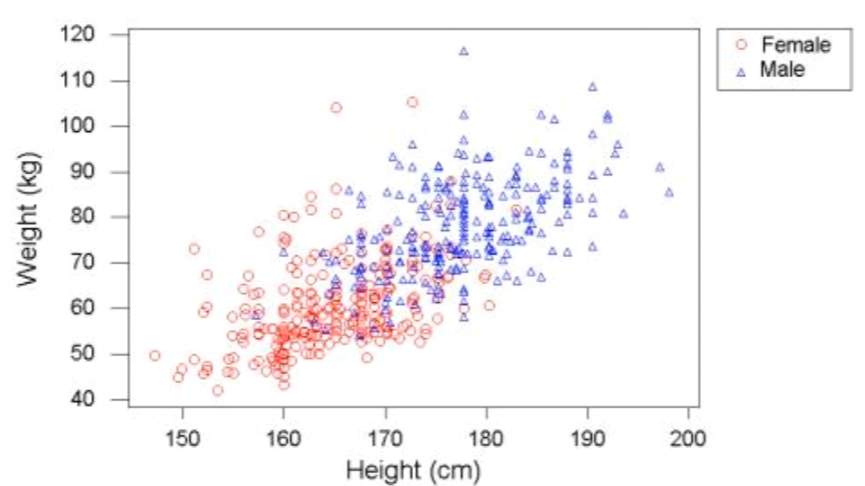
\includegraphics[height=0.6\paperheight ]{figures/cm2_notMagicClassification.png}
	\end{figure}

\end{frame}

\begin{frame}{Not magic, just geometry}
\begin{figure}
	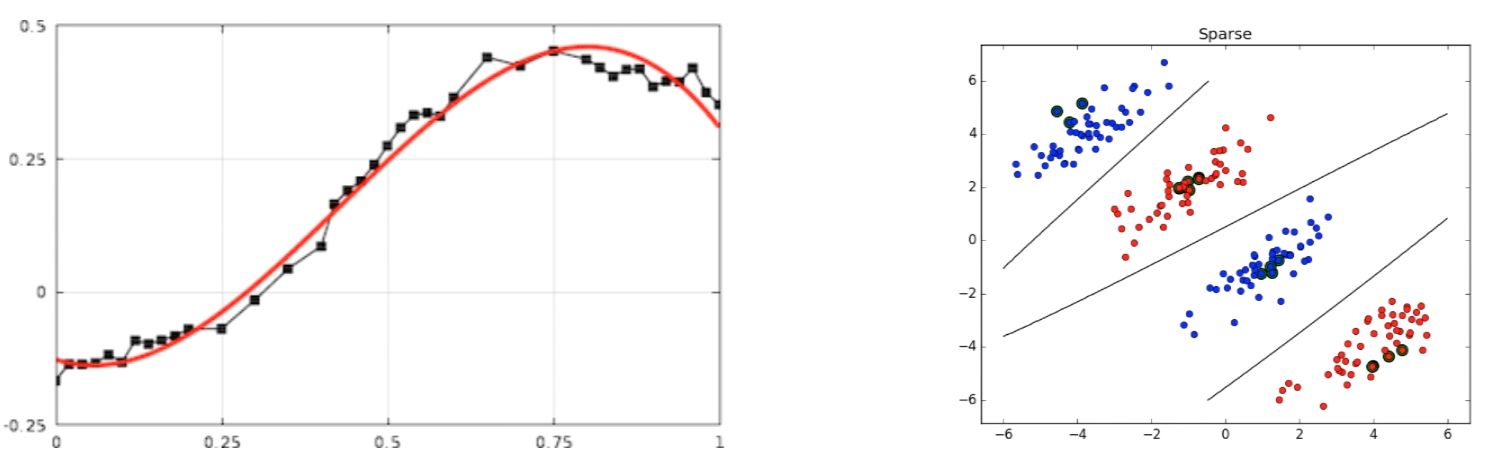
\includegraphics[height=0.45\paperheight ]{figures/cm2_notMagicClassification2.png}
\end{figure}
\begin{itemize}
	\item Regression cherche à trouver la courbe qui mieux décrit les caracteristiques des données
	\item Classification cherche la ligne qui sépare les données en fonction de ses caractéristiques.
\end{itemize}
\end{frame}

%------------------------------------------------
% Section divider frame
\makesection{Comparaison de modèles}
%------------------------------------------------


\begin{frame}{Toutes les interfaces sont les mêmes}
	\begin{itemize}
		\item Quel modèle choisir ?
		\item Les lignes de code sont les mêmes
		\item Pour quoi pas choisir le plus puissant, complexe, actuel, etc ?
		\item Il n'existe pas le modèle parfait.
		\item Cela dépend toujours des besoins.
		\item Pas de raccourci!!, il faut étudier les modèles
		\begin{itemize}			
			\item Apprendre leurs points faibles et forts
			\item Analyser les hyperparamètres
		\end{itemize}
	\end{itemize}
	
\end{frame}
%------------------------------------------------

\begin{frame}{Modèles linaires}
	\begin{itemize}
		\item Linear regression 
		\item Logistic regression 
		\end{itemize}
	\begin{figure}
		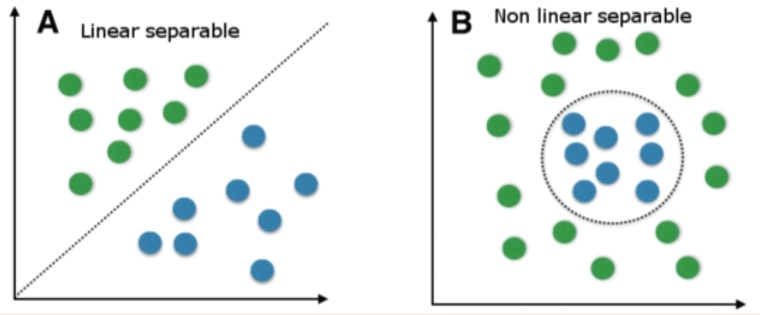
\includegraphics[height=0.4\paperheight ]{figures/cm2_LinealModels.png}
	\end{figure}
\end{frame}

%------------------------------------------------

\begin{frame}{Modèles linaires}
	\begin{itemize}
		\item Interprétation très simple
		\item au contraire des modèles non linaire
	\end{itemize}
	\begin{figure}
		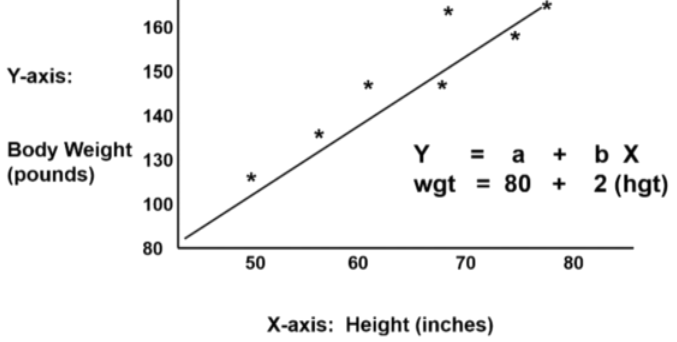
\includegraphics[height=0.5\paperheight ]{figures/cm2_LinealModels2.png}
	\end{figure}
\end{frame}


%------------------------------------------------

\begin{frame}{Modèles non linaires}
	\begin{itemize}
		\item Sont pas forcément les plus puissants
		\item Exemples : Bayes, Decision tree, K nearest neighbor
		\item Expérimenter avec plusieurs, sélectionner le meilleure ??
		\begin{itemize}
			\item L'importance de l'évaluation !
		\end{itemize}
	\end{itemize}

\begin{figure}
	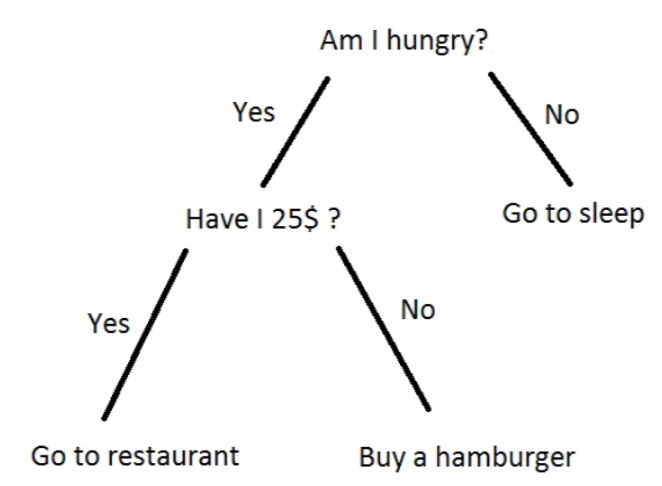
\includegraphics[height=0.5\paperheight ]{figures/cm2_notLinealModels.png}
\end{figure}
\end{frame}%------------------------------------------------

\begin{frame}{Modèles non linaires}
\begin{itemize}
	\item Sont pas forcément les plus puissants
	\item Exemples : Bayes, Decision tree, K nearest neighbor
	\item Expérimenter avec plusieurs, sélectionner le meilleure ??
	\begin{itemize}
		\item L'importance de l'évaluation !
	\end{itemize}
\end{itemize}

\begin{figure}
	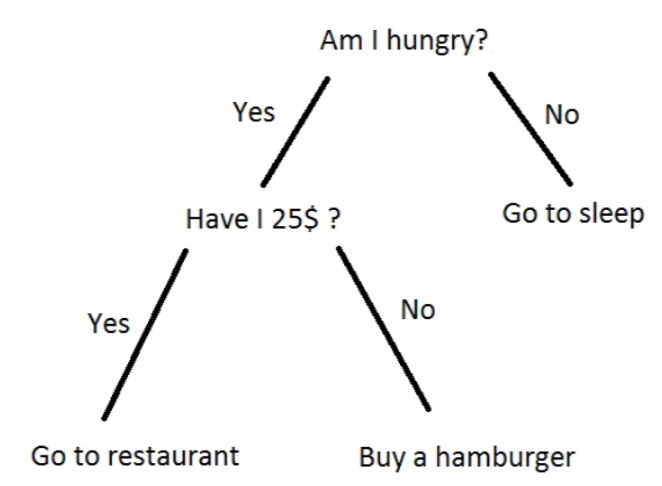
\includegraphics[height=0.5\paperheight ]{figures/cm2_notLinealModels.png}
\end{figure}
\end{frame}

%------------------------------------------------

\begin{frame}{Modèles fusionnés}
	\begin{itemize}
		\item Random forest, Ada Boost, ExtraTrees, Gradient Boosted, etc
		\item Construction d'un ensemble des modèles 
		\begin{itemize}
			\item Decision trees
			\item Calcul de la moyenne de prédiction
			\item Performance intéressante.
		\end{itemize}
		\item Très puissants, mais très coûteux.
		\item Netflix, Amazon ... 
	\end{itemize}
\end{frame}

%------------------------------------------------

\begin{frame}{SVM - Support Vector Machine}
	\begin{itemize}
		\item Considéré encore comme apprentissage profond 
		\item Plus performant que RN dans certains situations
		\item Puissant et non linaire
		\item MAIS il marche pas bien à échelle
		\begin{itemize}
			\item Besoin de toutes les données
			\item Actuellement el corpus sont immenses
			\item Implémentation coûteuse. 
		\end{itemize}
	\end{itemize}
\end{frame}

%------------------------------------------------
% Section divider frame
\makesection{Modèles pre entraînés}
%------------------------------------------------
\begin{frame}{Algorithmes}
	\begin{itemize}
		\item Des algorithmes existants sont disponibles.
		\begin{itemize}
			\item Traitement des données.
			\item Sélection de l'algorithme.
			\item Extraction des caractéristiques
			\begin{itemize}
				\item TD IDF
				\item Nb d'occurrences
				\item Proximité avec d'autres mots (analyse contextuelle)
			\end{itemize}
			\item Interface universelle de facile implémentation.
		\end{itemize} 
		\item Sci-kit learn
	\end{itemize}
	
\end{frame}

%------------------------------------------------
\begin{frame}{Pre traitement}
	\begin{itemize}
		\item Représentées dans une matrice 
		\begin{itemize}
			\item Colonnes [0 : N-1] = Caractéristiques (\textit{features})
			\item Colonne N = Étiquette (\textit{label ou target})
		\end{itemize} 
		\item Implémentation :
		\begin{itemize}
			\item Fréquence de mots - Nb d'occurrence d'un mot dans le document divisé par le nb total de mots dans le document par 100
			\item Deux étiquettes : 0= not spam 1= spam
		\end{itemize} 
		\item Les colonnes représentent les mots, les lignes représentent les documents.
		\item Ceci est juste un exemple d’implémentation !
	\end{itemize}
	
\end{frame}


%------------------------------------------------
\begin{frame}{Pre TD1}
	Let's code !
	%Section 3; video 9
	
\end{frame}

%------------------------------------------------
% Section divider frame
\makesection{Questions ?!}

%------------------------------------------------
% Section divider frame
\makesection{TD-1 ! Classification de textes}


%------------------------------------------------
% Lists
\begin{frame}{Classificateur}
	\begin{itemize}
		\item Question ... 
		\item Étant donné un poème, pouvons-nous savoir à quel auteur il appartient ?
		\item Input(texte) -> Classifier() --> est-ce que c'est un poème d'Allan Poe ?
	\end{itemize}

	\vspace{0.5cm}
	
	\textbf{Autres exemples}	
	\begin{itemize}
		\item E-mail
		\begin{itemize}
			\item Spam or not spam
		\end{itemize}
		\item Critique d'un film
		\begin{itemize}
			\item Positif ou négatif 
		\end{itemize}
	\end{itemize}
	
\end{frame}

%------------------------------------------------
% Lists
\begin{frame}{Problématique}
	\begin{itemize}
		\item Classification de textes, une tâche des méthodes non supervisées
		\item Markov tolère que de texte, pas d’étiquettes.
		\item Comment résoudre le problème ?
			\begin{itemize}
				\item \textbf{Naïve Bayes}
				\item ... Building a Bayes classifier based on rules
			\end{itemize}
	\end{itemize}
	
	\begin{figure}
		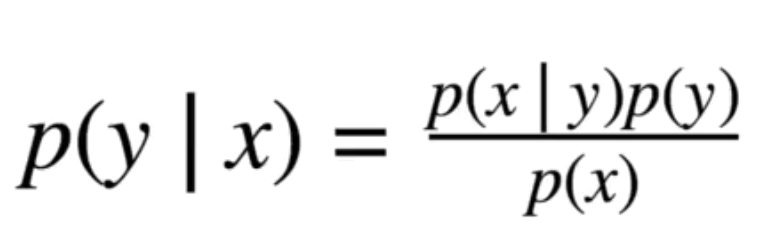
\includegraphics[height=0.25\paperheight]{figures/eq1.png}
	\end{figure}
	
\end{frame}

%------------------------------------------------
% Lists
\begin{frame}{Étape d'entraînement - $A$ et $\pi$ }
	\begin{itemize}
		\item Entraîner les modèles linguistiques nécessaires ... une par Classe.
		\begin{itemize}
			\item Définir et calculer $A$ et $\pi$ 
			\item ... Building a Bayes classifier based on rules
		\end{itemize}
		\item À partir de $A$ et $\pi$, et une séquence ${s_1,s_2,...s_T}$. Quelle est la probabilité de trouver cette séquence ?
		
		\item Comment calculer $A$ et $\pi$ ?
	\end{itemize}
	
	\begin{figure}
		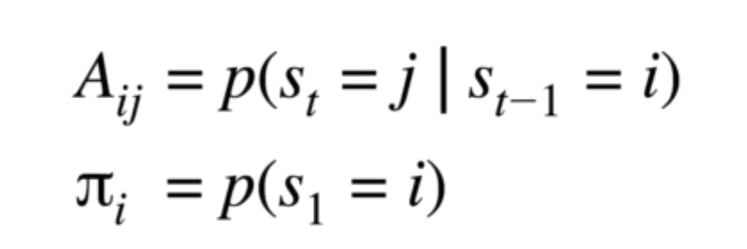
\includegraphics[height=0.25\paperheight]{figures/eq1AnPi.png}
	\end{figure}
	
\end{frame}



%------------------------------------------------
% Lists
\begin{frame}{Étape d'entraînement - les séquences}
	\begin{itemize}
		\item Entraîner les modèles linguistiques nécessaires ... une par Classe.
		\begin{itemize}
			\item Définir et calculer $A$ et $\pi$ 
			\item ... Building a Bayes classifier based on rules
		\end{itemize}
		\item \textbf{ À partir de $A$ et $\pi$, et une séquence ${s_1,s_2,...s_T}$. Quelle est la probabilité de trouver cette séquence ?}
	\end{itemize}
	
	\begin{figure}
		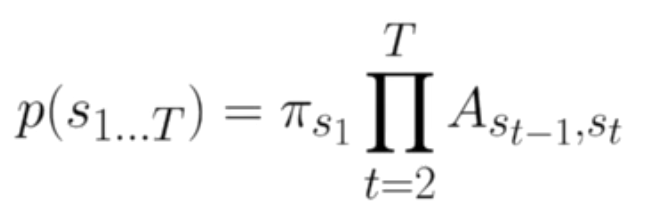
\includegraphics[height=0.2\paperheight]{figures/eqSeqMult.png}
	\end{figure}
	
	\begin{itemize}
		\item C'est que la multiplication des valeurs des transitions calculées.
		\item Si une de ces valeurs est $0$ ? Une transition jamais vue.
		\item Tout devient $0$
	\end{itemize}
	
\end{frame}

%------------------------------------------------
% Lists
\begin{frame}{Étape d'entraînement - $\hat{A}$ et $\hat{\pi}$}
	\begin{itemize}
		\item Entraîner les modèles linguistiques nécessaires ... une par Classe.
		\begin{itemize}
			\item Définir et calculer $A$ et $\pi$ 
			\item ... Building a Bayes classifier based on rules
		\end{itemize}
		\item À partir de $A$ et $\pi$, et une séquence ${s_1,s_2,...s_T}$. Quelle est la probabilité de trouver cette séquence ?
		
		\item \textbf{Comment lisser  $A$ et $\pi$ ?}
	\end{itemize}

	\begin{figure}
		\centering
		\begin{subfigure}{.5\textwidth}
			\centering
			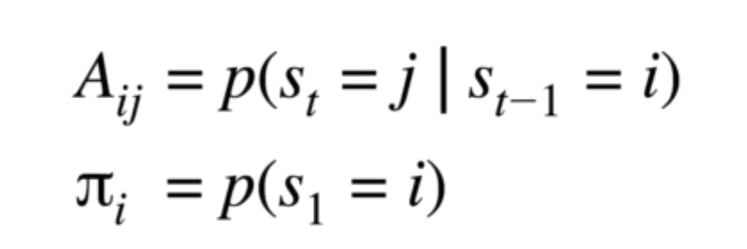
\includegraphics[width=0.78\linewidth]{figures/eq1AnPi.png}
			\caption{Version classique}
		\end{subfigure}%
		\begin{subfigure}{.5\textwidth}
			\centering
				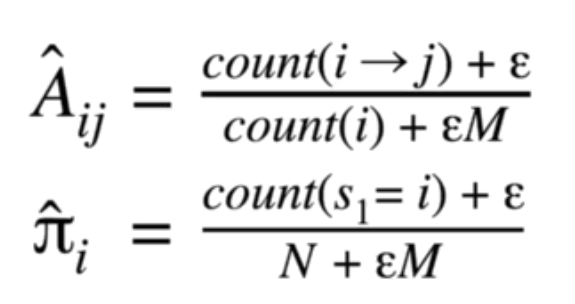
\includegraphics[width=0.48\paperheight]{figures/eq1AnPiEst.png}
			\caption{Estimation de $A$ et $\pi$}
		\end{subfigure}
	\end{figure}
	
\end{frame}


%------------------------------------------------
% Lists
\begin{frame}{Étape d'entraînement - smoothing}
	\begin{itemize}
		\item Entraîner les modèles linguistiques nécessaires ... une par Classe.
		\begin{itemize}
			\item Définir et calculer $A$ et $\pi$ 
			\item ... Building a Bayes classifier based on rules
		\end{itemize}
	\end{itemize}
	
	\begin{figure}
		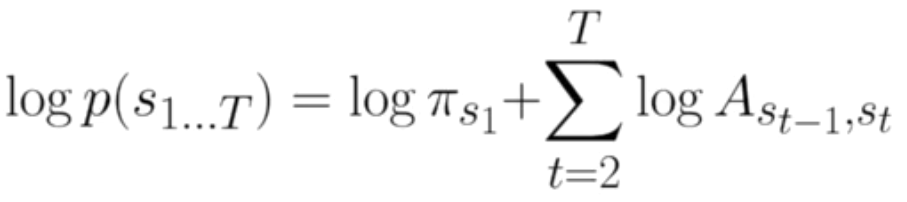
\includegraphics[height=0.2\paperheight]{figures/eqSmoothed.png}
	\end{figure}

	\begin{itemize}
		\item Nous remplaçons la multiplication pour somme (Simplification)
		\item On garde que les logged values car arg max needed
		\item Respectez l'ordre : log() and then sum()
	\end{itemize}
	
\end{frame}

%------------------------------------------------
% Lists
\begin{frame}{Fonctionnement}
\begin{itemize}
	\item Étant donné les objets $A$ et $\pi$ et un texte comme input
	\item ... calculer la probabilité que ce texte appartienne a la classe analysée
\end{itemize}

\begin{figure}
	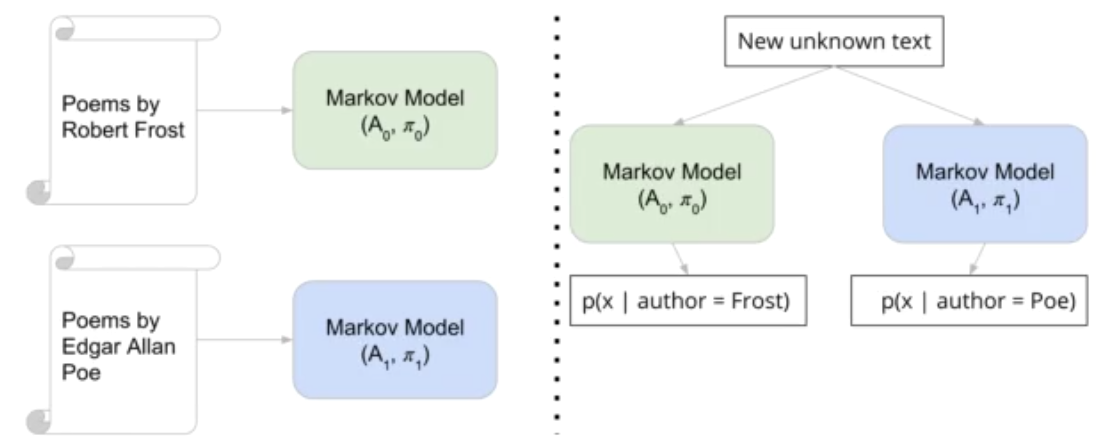
\includegraphics[height=0.5\paperheight]{figures/img1.png}
\end{figure}


\end{frame}

%------------------------------------------------
% Lists
\begin{frame}{Les règles...}
	\begin{itemize}
		\item On a \textit{p(poème|auteur)} mais on a besoin de \textbf{\textit{p(auteur|poème)}}
		\item Nous devons donc appliquer l'équation :
	\end{itemize}
	
	\begin{figure}
		\centering
		\begin{subfigure}{.5\textwidth}
			\centering
			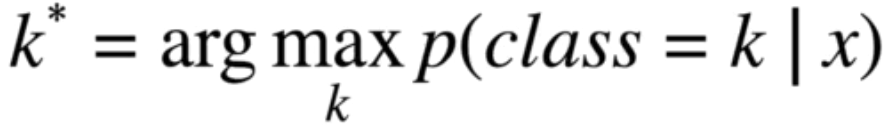
\includegraphics[width=0.7\textwidth]{figures/eq2.png}
		\end{subfigure}%
		\begin{subfigure}{.5\textwidth}
			\centering
			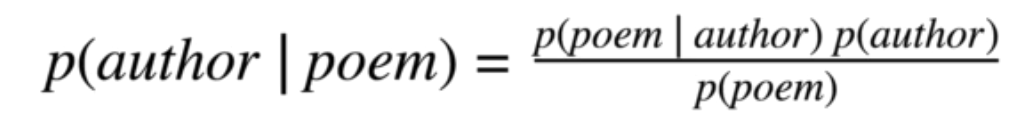
\includegraphics[width=0.8\textwidth]{figures/eq3.png}
		\end{subfigure}
		\textbf{Si l'on simplifie l'équation}
		\begin{figure}
			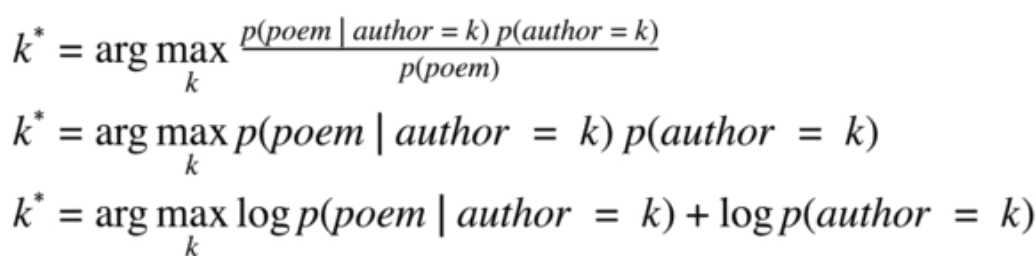
\includegraphics[width=0.7\textwidth]{figures/img2.png}
		\end{figure}
	\end{figure}

\end{frame}



%------------------------------------------------
% Section divider frame
\makesection{TD-2 ! Génération de textes}

%------------------------------------------------

%------------------------------------------------
% Lists
\begin{frame}{Modèle génératif}
	\begin{itemize}
		\item Classification de textes : supervisé (étiquettes)
		\begin{itemize}
			\item Discriminatif
			\item $p(y|x)$
		\end{itemize}
		\item Générateur de textes : non supervisé (pas d'étiquettes)		\begin{itemize}
			\item Génératif
			\item $p(x|y)$
		\end{itemize}
			
	\end{itemize}		
\end{frame}


\begin{frame}{\textit{Sampling} ... }
	\begin{itemize}
		\item Sampling avec N(0,1) : \textit{np.random.randn()}
		\item Sampling avec Bernouli : \textit{np.random.choice([0,1])}
		\item Bernouli avec p(heads=0.8) (où heads = 1) :
		\begin{itemize}
			\item \textit{np.random.choise([0,1] , p=[0.2 , 0.8])}
		\end{itemize} 
	\end{itemize}
	\vspace{0.5cm}
	\textbf{Sampling words} - Supposons que nous avons un vocabulaire = ('cat', 'dog', 'mouse')
	\begin{itemize}
		\item Avec leurs probabilité d'apparition : (0.2, 0.5, 0.3)
		\item Si l'on peut cartographier le vocabulaire  comme (1, 2, 3), ça devient facile
		\begin{itemize}
			\item \textit{np.random.choice(3, p=[0.2, 0.5, 0.3])}
		\end{itemize}
		
	\end{itemize}		
\end{frame}

%------------------------------------------------

\begin{frame}{Problématique}
	Rappelez que le mot prochain dépend uniquement du mot précédent
	\begin{examples}
		\begin{enumerate}
			\item Je me suis préparé moi-même un sandwich au beurre.
			\item Je vais aller lui rendre visite moi-même.
		\end{enumerate}
		\begin{itemize}
			\item \textbf{ Je vais aller lui rendre visite moi-même un sandwich au beurre.}
		\end{itemize}
	\end{examples}

	\begin{examples}
		\begin{enumerate}
			\item Je me suis préparé moi-même un sandwich au beurre.
			\item Le beurre n'est pas une noisette
		\end{enumerate}
		\begin{itemize}
			\item \textbf{ Je me suis préparé moi-même un sandwich au beurre n'est pas une noisette.}
		\end{itemize}
	\end{examples}
\end{frame}
%------------------------------------------------

\begin{frame}{Prolongement du modèle de Markov}
	
	\begin{itemize}
		\item Au lieu d'observer que le mot précédent : 
		\begin{itemize}
			\item Markov de premier ordre
			\item $p(s_t |s_{t-1}, s_{t-2}, ...) = p(s_t | s_{t-1})$
		\end{itemize}
		\item ...on observe les deux mots précédent
		\begin{itemize}
			\item Markov de premier ordre
			\item $p(s_t |s_{t-1}, s_{t-2}, ...) = p(s_t | s_{t-1}, s_{t-2})$
		\end{itemize}
		\item \textit{Afin de mieux prédire le future, il faut mieux observer le passé}
	\end{itemize}

\end{frame}

%------------------------------------------------

\begin{frame}{Modèle complet}
	
	\begin{itemize}
		\item $ \pi_i = p(s_1 = i)$
		
		\item $ A^{(1)}_{ij} = p(s_2 = j | s_1 = i)$
		
		\item $ A^{(2)}_{ijk} = p(s_t = k | s_{t-1}, s_{t-2} = i)$
	\end{itemize}

\begin{example}
	"The quick brown fox jumps over the lazy dog" \\
	"\textbf{The}" -> $\pi$\\
	"\textcolor{red}{The} \textbf{quick}"-> $A^{(1)}$\\
	"\textcolor{red}{The quick} \textbf{brown} " -> $A^{(2)}$\\
	"The \textcolor{red}{quick brown} \textbf{fox} " -> $A^{(2)}$\\
\end{example}
	
\end{frame}

%------------------------------------------------
% Refenrenced
\begin{frame}{Références}
    % Beamer does not support BibTeX so references must be inserted manually as below
    \footnotesize{
        \begin{thebibliography}{99}
            \bibitem[Bento, 2020]{p1} Carolina Bento (2020)
            \newblock Markov models and Markov chains explained in real life: probabilistic workout routine
            \newblock \href{https://towardsdatascience.com/markov-models-and-markov-chains-explained-in-real-life-probabilistic-workout-routine-65e47b5c9a73}{https://towardsdatascience.com/markov-models-and-markov-chains-explained...}
            
            \bibitem[Bento, 2020]{p1} Pat Brans (2022)
            \newblock What is a Markov model?
            \newblock \url{https://www.techtarget.com/whatis/definition/Markov-model}

            \bibitem[Bento, 2020]{p1} Wikipedia free encyclopedia (2024)
            \newblock Markov model
            \newblock \url{https://en.wikipedia.org/wiki/Markov_model}
            
            %\bibitem[Doe, 2013]{p} Jane Doe (2012)
            %\newblock Title of the publication
            %\newblock \emph{Journal Name} 12(3), 45 -- 678.
        \end{thebibliography}
    }
\end{frame}

%----------------------------------------------------------------------------------------
% Final PAGE
% Set the text that is showed on the final slide
\finalpagetext{Thank you for your attention}
%----------------------------------------------------------------------------------------
\makefinalpage
%----------------------------------------------------------------------------------------
\end{document}